\documentclass[9pt,a4paper]{report}
\usepackage{mwe}
\usepackage{listings}
\usepackage{amsmath}
\usepackage{graphicx}
\usepackage{subfig}
\usepackage{float}
\usepackage{xcolor}
\usepackage{multirow}
\usepackage{hyperref}
\usepackage{fancyhdr}
\usepackage{sectsty}
\usepackage[dvipsnames]{xcolor}
\usepackage{soul}
\usepackage[compact]{titlesec}
\usepackage{float}
\usepackage[left=0.5cm,right=0.5cm,top=0.5cm,bottom=0.5cm]{geometry}
\graphicspath{{Series Forward-Bias Diode Circuit}}

\newcommand*{\nchapter}[1]{%
	\chapter*{#1}%
	\addcontentsline{toc}{chapter}{#1}
	\vspace{-14mm}}
\newcommand*{\nsection}[1]{%
	\section*{#1}%
	\addcontentsline{toc}{section}{#1}}
\newcommand*{\nsubsection}[1]{%
	\subsection*{#1}%
	\addcontentsline{toc}{subsection}{#1}}
\newcommand*{\nsubsubsection}[1]{%
	\subsubsection*{#1}%
	\addcontentsline{toc}{subsubsection}{#1}}

\chaptertitlefont{\large}
\sectionfont{\normalsize}
\fontsize{9}{11}\selectfont
\begin{document}
	\begin{titlepage}
		\centering
		\vspace*{1.5in}
		
\includegraphics[width=0.15\textwidth]{W-Logo_Purple_RGB}\par\vspace{1cm}
		{\LARGE \textsc{University of Washington}\par}
		\vspace{1cm}
		{\Large \textsc{BEE331 Lab 1.1}\par}
		\vspace{1.5cm}
		{\huge\bfseries \par}
		\vspace{2cm}
		{\Large\itshape 2301991\hspace{55pt}2130474\par}
		{\Large\itshape Jason Truong\hspace{31pt}Henry Haight\par}
		\vfill
		supervised by\par
		Prof.~Joseph \textsc{Decuir}
		\date{2024\\ January}
		\vfill
		% Bottom of the page
		{\large \today\par}
		\vspace*{1.5in}
	\end{titlepage}
	
	\nchapter{Characterising Diodes; I-V Curve}
	\nsection{Design Objective}
	In this lab, we introduce ourselves to the diode, we characterise its function by the I-V curve.
	\begingroup
	\renewcommand{\cleardoublepage}{}
	\renewcommand{\clearpage}{}
	\nsection{Circuit Design Outline}
	\endgroup
	With a resistor of an arbitrary impedance greater than $50\Omega$ ($R\geq100\Omega$), and the natural impedance of the Function Generator in series ($R_{TOT}=R_{FG}+R\geq150\Omega$), the (1N4148 silicon) diode is set in series to forward-bias from the function generator. Set the function generator @ f=1kHz and $V_P=5V$.
	\begin{figure}[hpb!]
		\centering
		\caption{\centering RLC Circuit}
		\subfloat[\centering LTSpice + Rudimentary Schematic RLC Circuit]{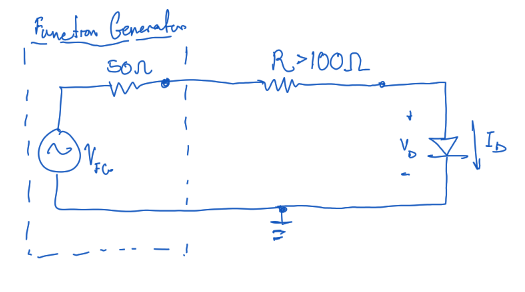
\includegraphics[width=10cm]{image}}\hfil
		\subfloat[\centering RLC Circuit]{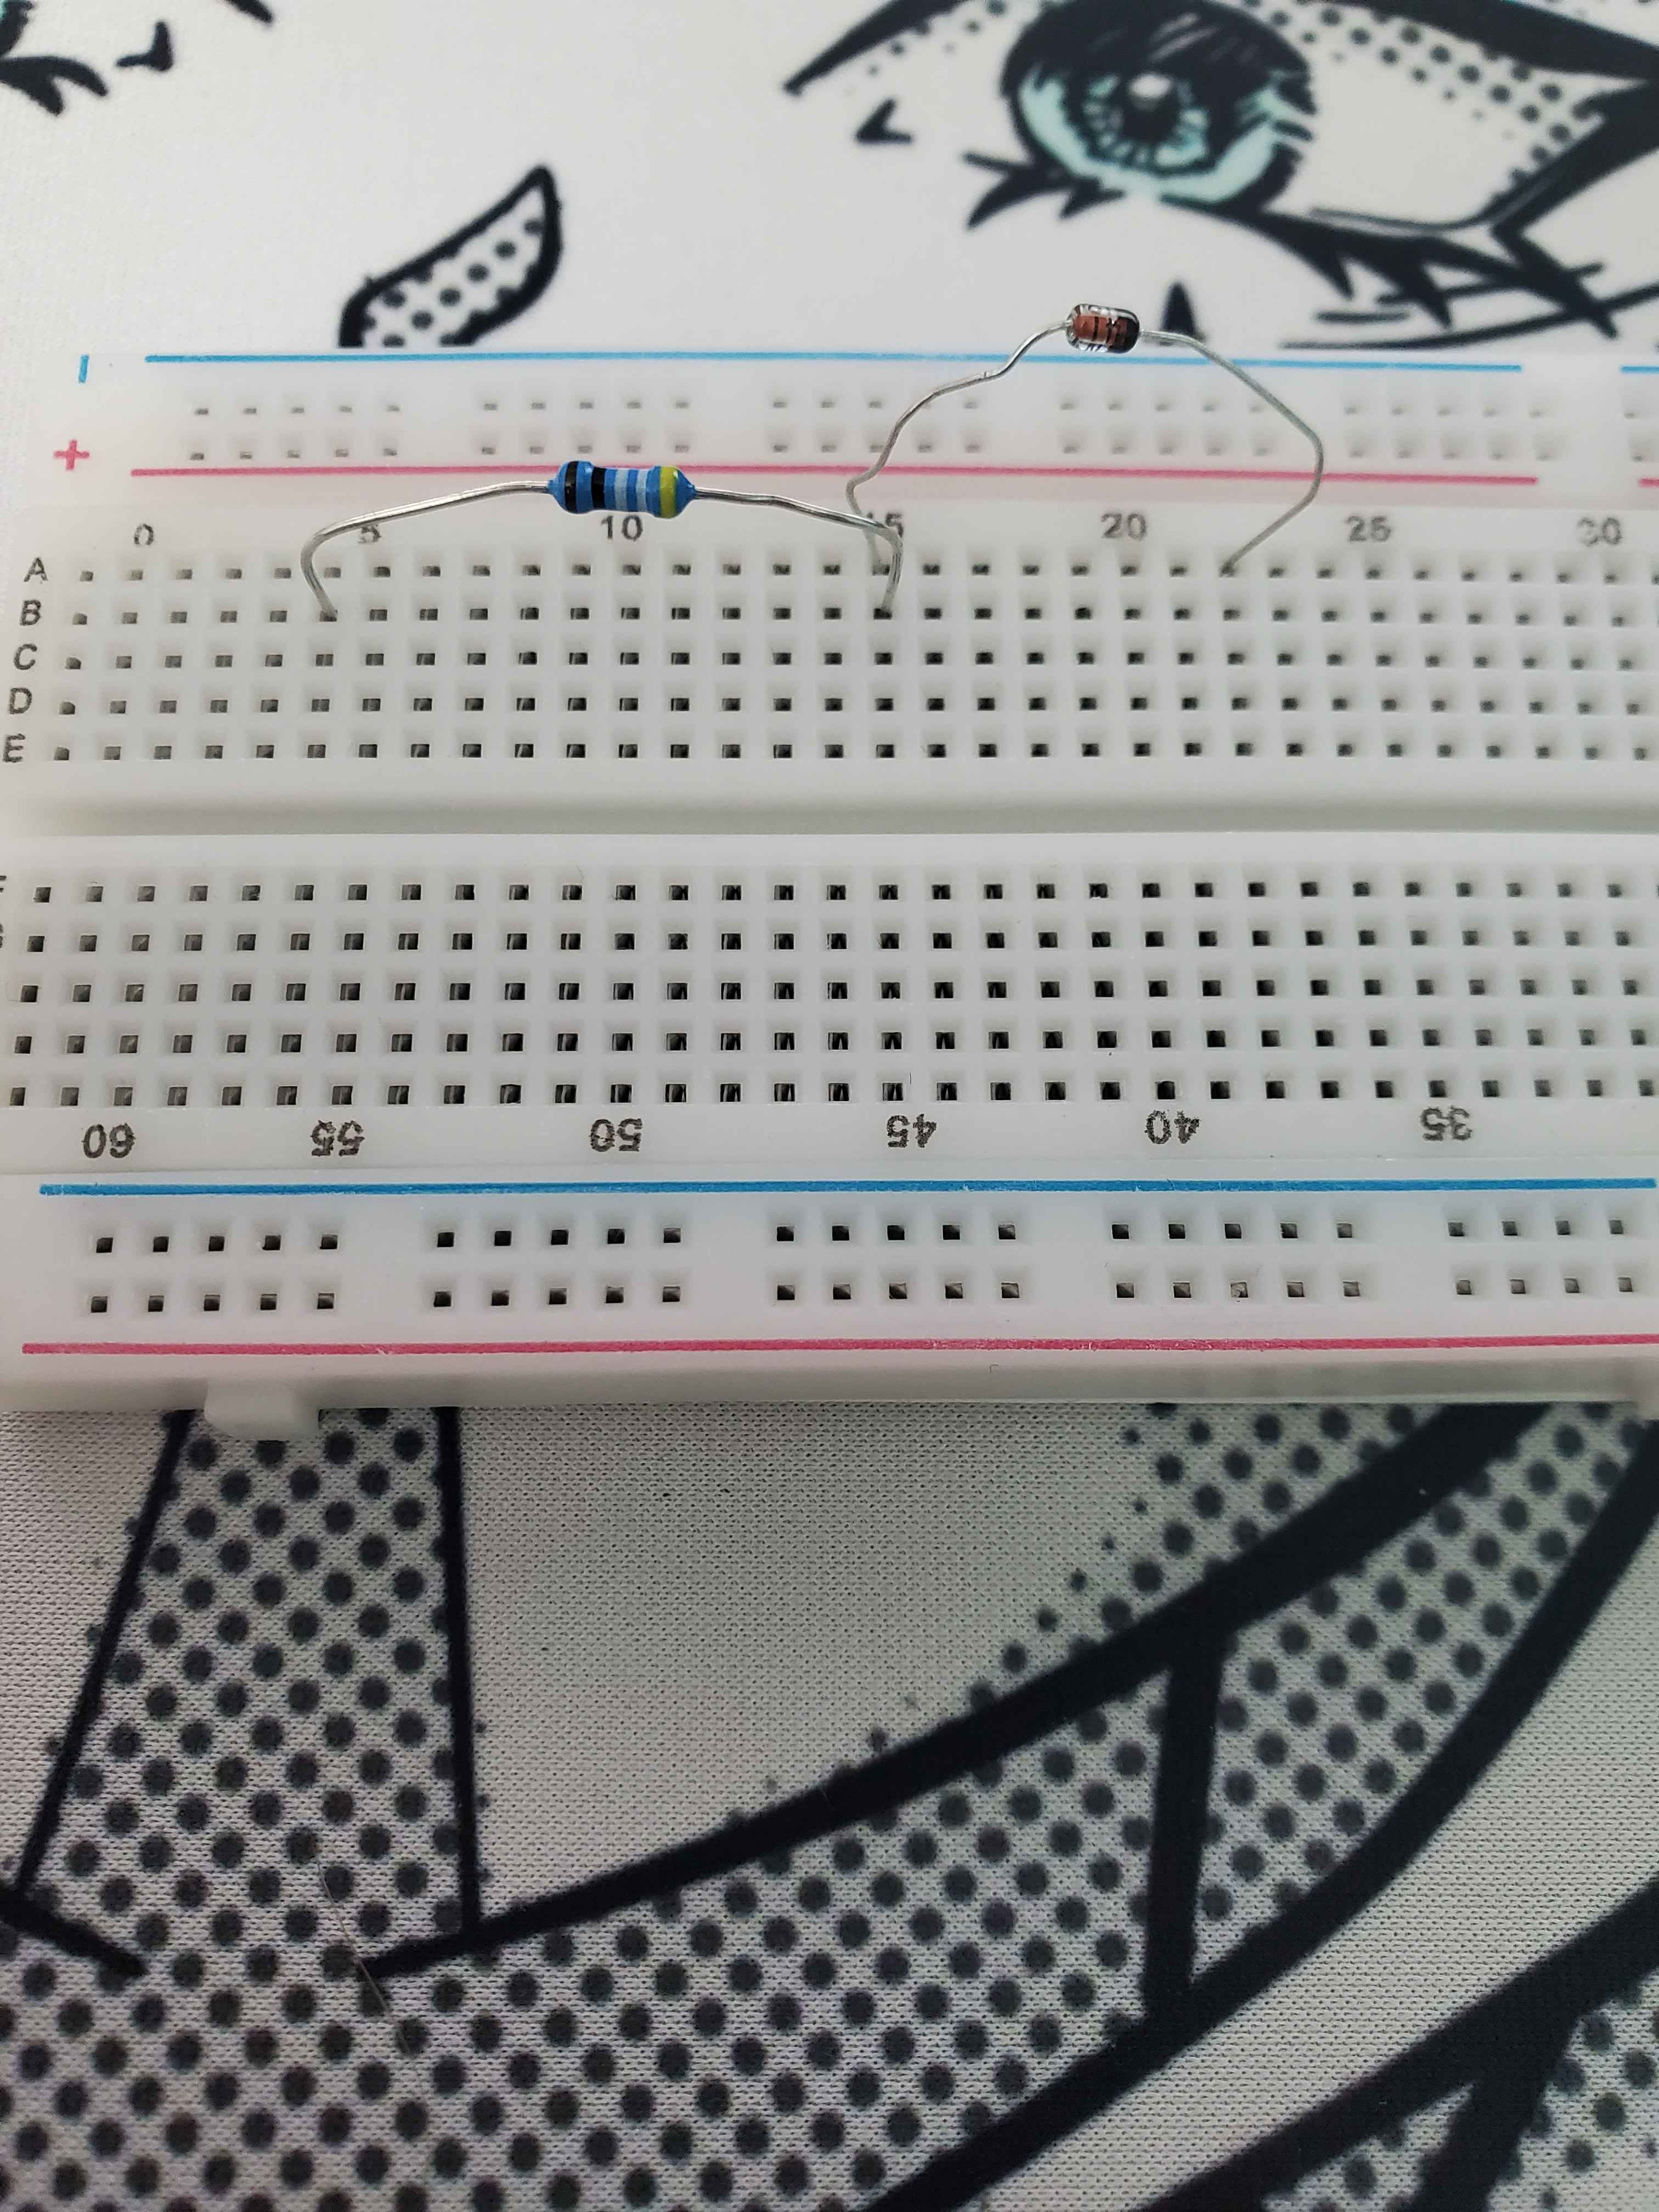
\includegraphics[width=10cm]{20240714_094126}}
	\end{figure}
	\nsection{Descriptions of Measurements \& Calculations}
	Anylsing the data below, the measured and LTSpice sim were similar. Except the LTSpice sim had a measured rise-time much lower than the LTSpice calculations.
	\begin{figure}[hp!] %140, 
		\centering
		\caption{RLC Circuit}
		\subfloat[RLC Circuit: Math]{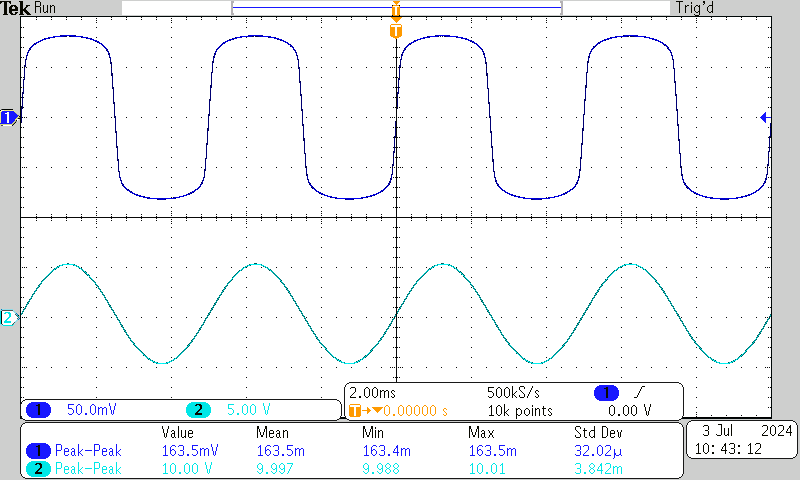
\includegraphics[width=10cm]{tek0001}}\hfil
		\subfloat[Square RLC Circuit]{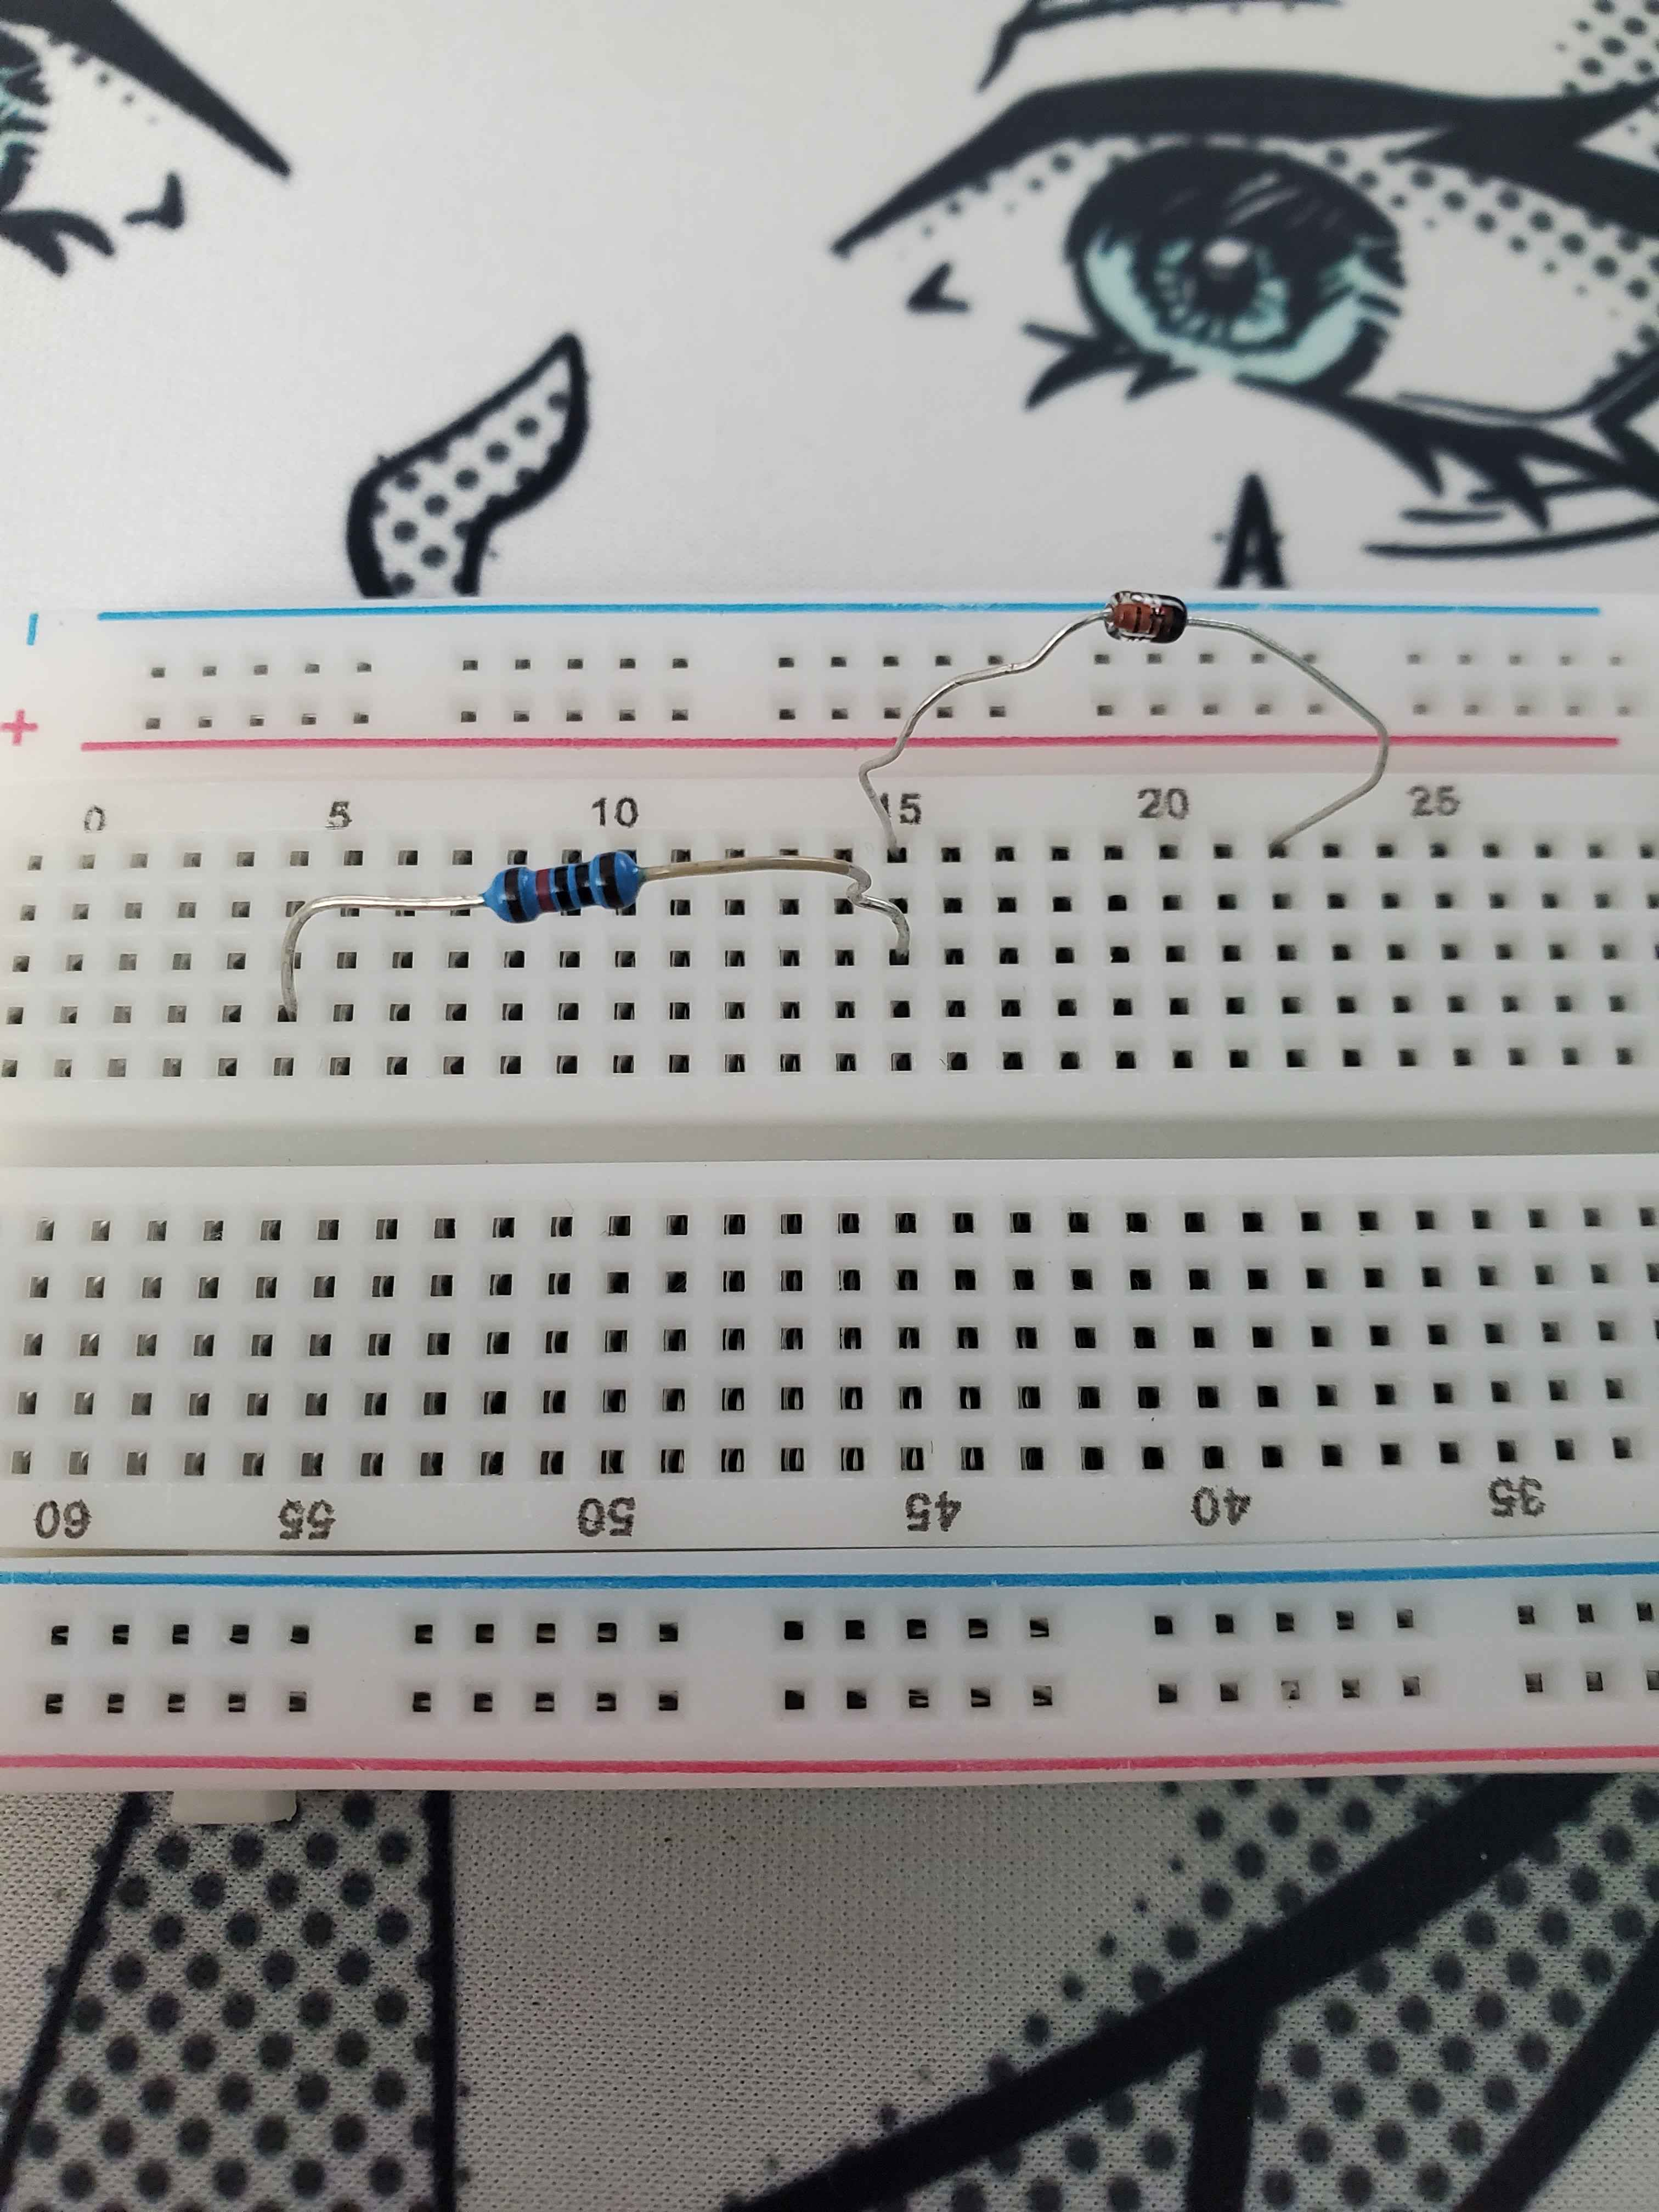
\includegraphics[width=10cm]{20240714_094141}}\hfil
	\end{figure}
	\nsection{Summary \& Conclusions}
	Revealed in Figure 2(a-b), the primary components; the Inductor and Capacitor, overcompensate and overdamp the circuit, and grew to be greater than the voltage originally. The calculation and the measurements in actuality were very close in similar measurements.
	\newpage
	\nchapter{Addendum Pages}
	\begin{figure}[hp!]
		\centering
		\caption{Jason Truong Addendum}
		\subfloat[\centering Lab Design   Calculations]{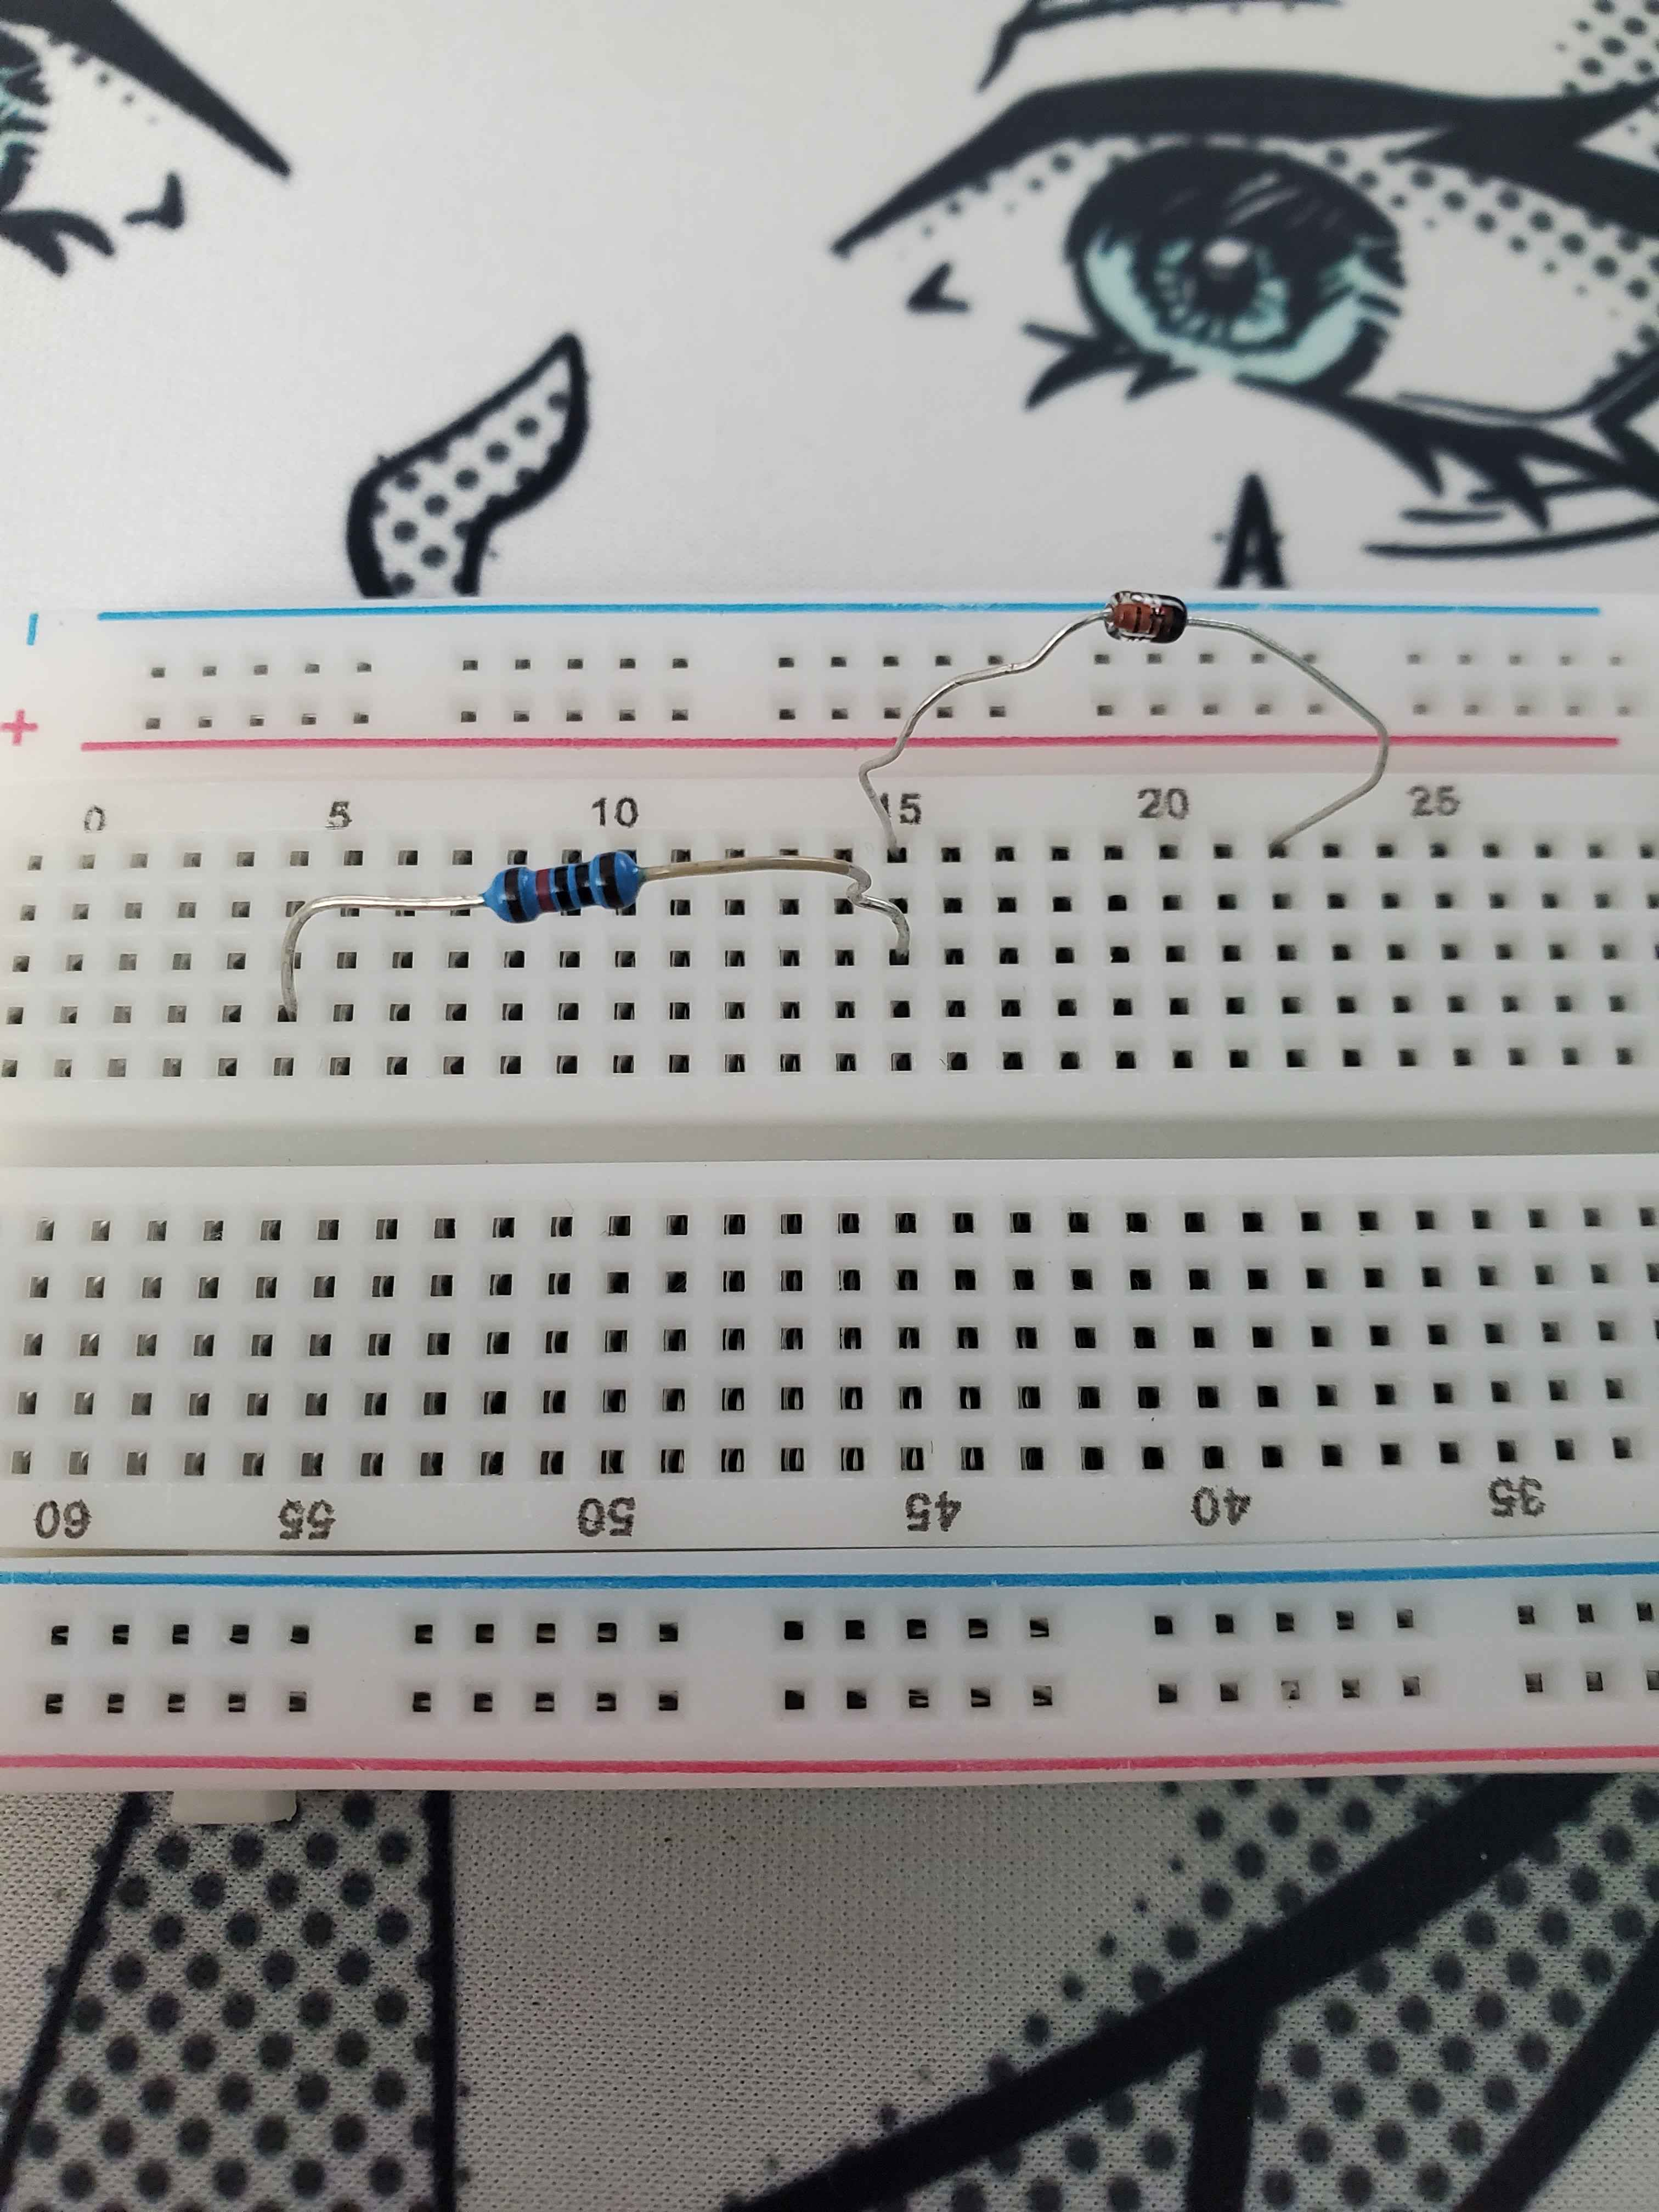
\includegraphics[width=17cm]{20240714_094141}}
	\end{figure}
	\newpage
	\nsection{Bibliography}
	\textbf{Cited:}\\
	\begin{itemize}
		\item Lab 1 Manual
		\item Class textbook: "Electric Circuits 11e, Nillson \& Riedel"
	\end{itemize}
	\begin{figure}[!h]
		\subfloat[Look at her, she's perfect.]{
\includegraphics[width=\linewidth]{GodILoveFurina}}
	\end{figure}
\end{document}